\chapter{Proposed Model} \label{ch:Ch.4}
After analyzing the $BRI_2$ in the previous chapter, the proposed model will be presented. In particular, this chapter will describe in detail the model implemented starting from the dataset used and the pre-processing techniques to the chosen architecture. The goal of the model is to provide a daily risk-index based on the observations of the previous days. In particular, given an airport, the model looks at a window of $K$ days and provides the risk-value for the following day. 

\section{Dataset}
The dataset used includes data from more than 100 Italian airports, including military airports and internal divisions dedicated to internal and external naturalistic research. Data quality varies from airport to airport.
The dataset includes all daily data that derives from the Bird Strike Reporting Form, which is divided into Impact Reporting Form and Fauna Monitoring Form \cite{ENAC-Wildlifestrike}. In particular:

\begin{itemize}
    \item Impact Reporting Form: Includes all data related to birdstrike such as including effect on flight, number of animals involved, weather, flight phase etc.
    \item Fauna Monitoring Form: Includes all data related to daily inspections done at airports such as number of daily sightings, weather conditions, temperature, wind intensity and direction, area of sighting etc.
\end{itemize}
In addition, the dataset also provides a number of movements, i.e. monthly landing and take-off data.
The data was provided in the form of a database of raw data, the BirdControl DBMS. 


\section{Data Pre-processing}
This section will show the techniques of data pre-processing used to manage the raw data in order to input them into the model.
In fact, much of the data in the database shown is missing, incomplete or with inconsistent values and not all the data is relevant.
In this case, features selection and data cleaning are the first and most important step of the model design.

\subsection{Feature selection}
Features selection is one of the core concepts in Machine Learning which hugely impacts on the performance of the implemented model.
For this work it was very important to choose features that could explain the behaviour of the model in order to interpret the new risk-index according to the input features as much as possible.

The first feature selected was Sighted Species. It is one of the most important features on which the model is based on and it's important because the higher the number of sightings, the more likely it is that a wildlife strike event will occur. The division into species has been maintained so that the model understands which sightings are more dangerous over time.
To add more information to the sightings, the distance to the track and the detection environment have been added; contributing to the best accuracy of the model.

The next features have been chosen according to the biology and ecology of the birds in order to describe their behaviour and habits, for this reason Meteorological Conditions, Temperature, Wind Direction, Wind Intensity and Presence of Wet Ground have been selected.
The number of birdstrikes has also been entered. It refers to the number of birdstrikes in the days before the one in which the risk value is to be provided.
This choice was made after an analysis of the birdstrikes that have historically occurred and it was found that at certain periods of the year there is a greater tendency for them to happen.
For example you can see in Figure \ref{bird_distrib} the distribution of all verified birdstrike events remapped in a single year.
Since the occurrence of birdstrikes has a seasonal trend the number of birdstrikes of the previous days as well as of the previous year has also been included.
\begin{figure}
	\centering
	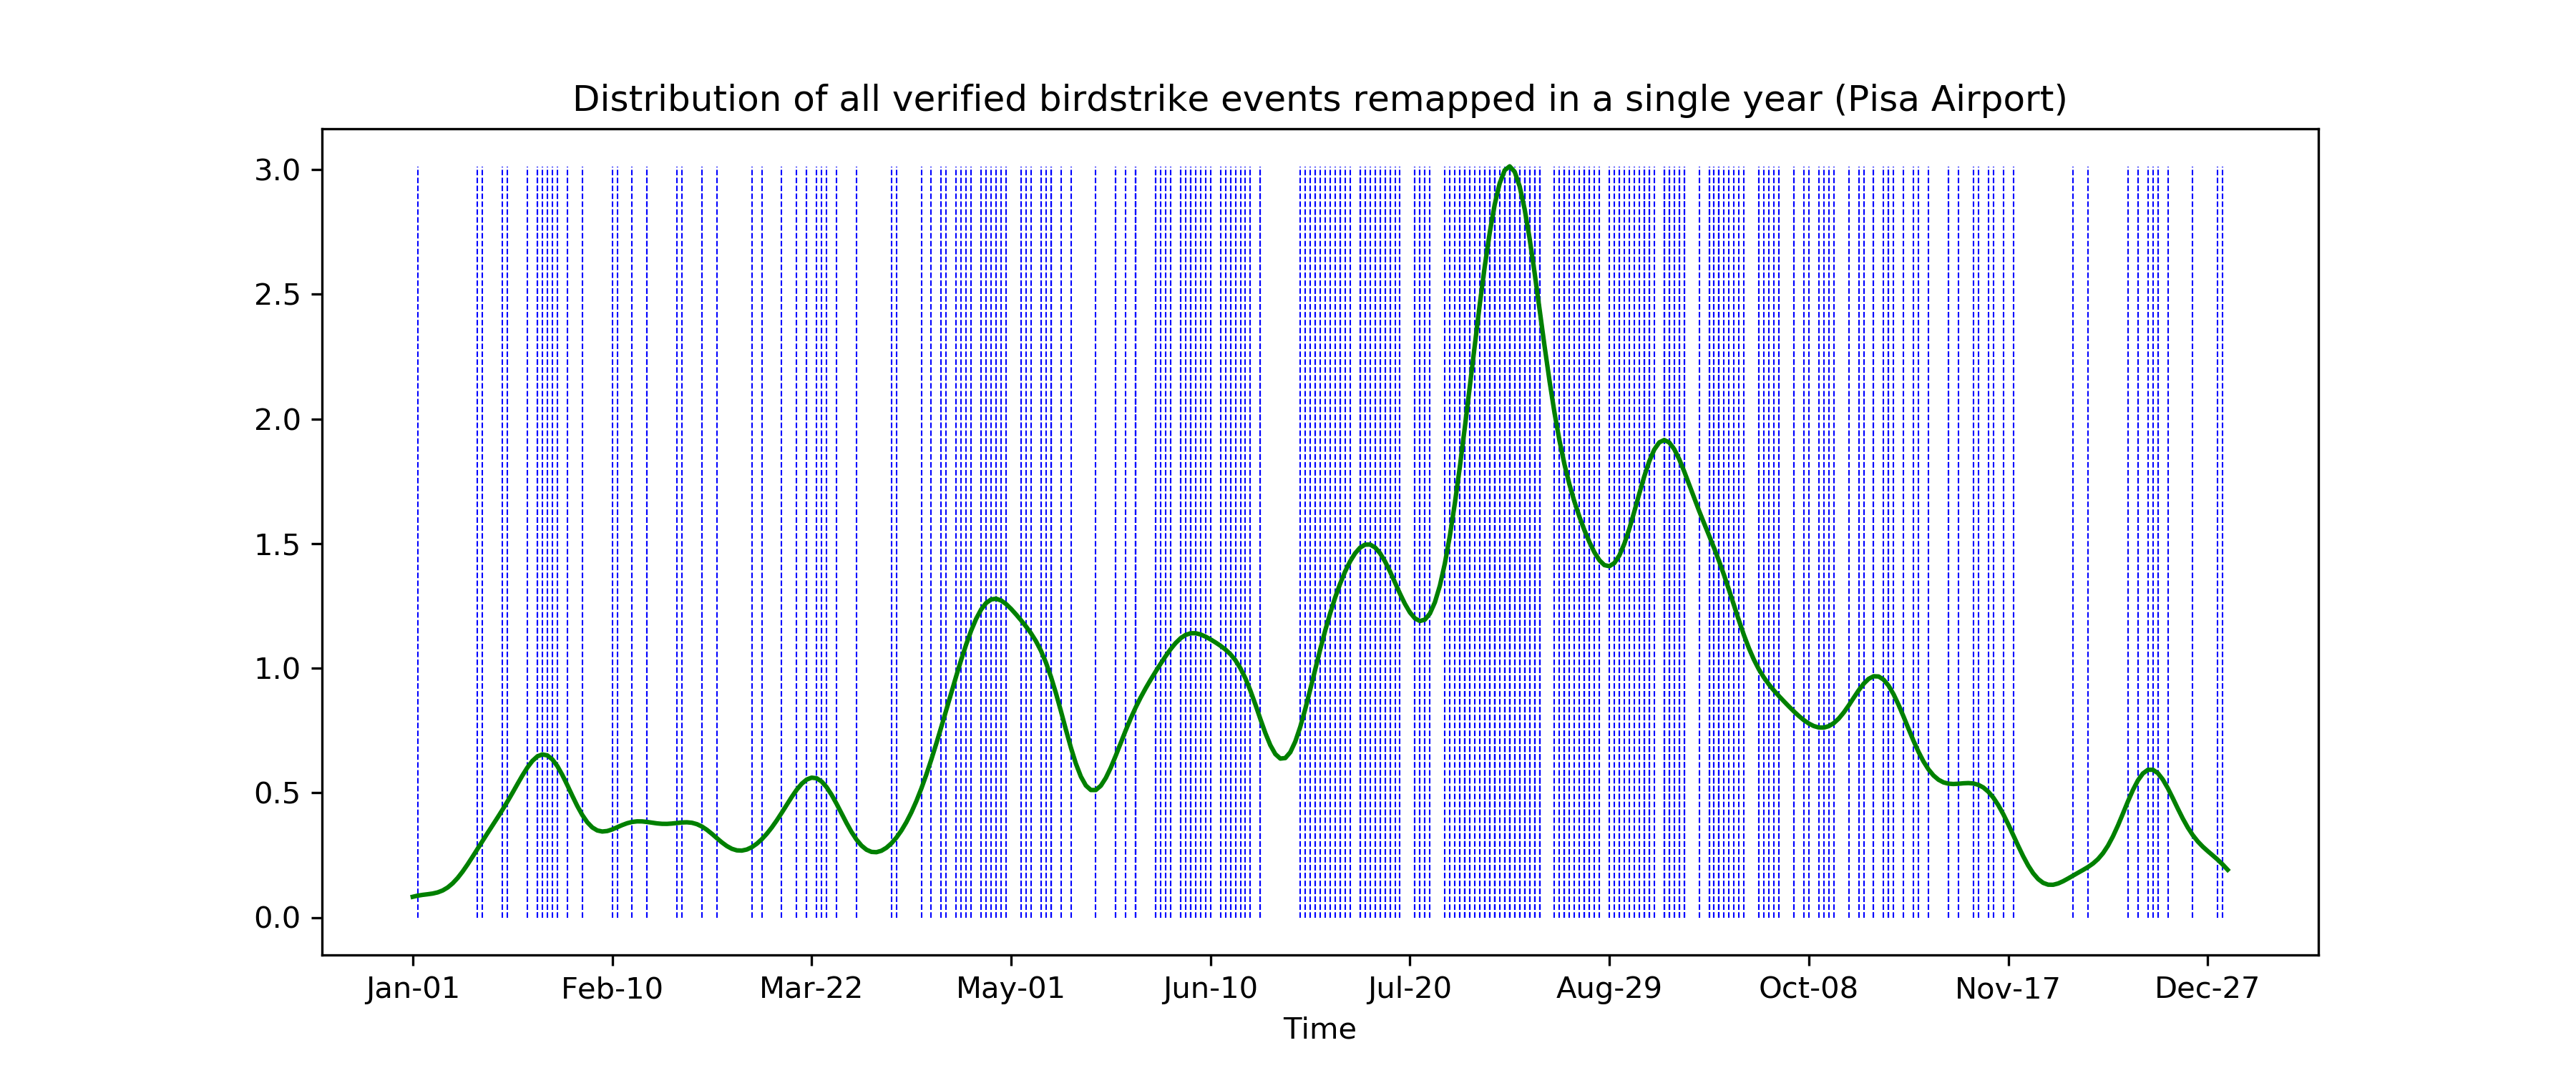
\includegraphics[width=13.8cm]{img/plot_distrib.png}
	\caption{Distribution of all verified birdstrike events remapped in a single year for Pisa Airport. The figure shows how the historical events of birdstrike collected are present all year long but focusing more on a specific period, from June to October indicating a seasonal trend}
	\label{bird_distrib}
\end{figure}
The number of birdstrikes and birdstrikes of the previous year have contributed significantly to the model's performance, considerably increasing the correlation between the new risk index and birdstrike events.

\subsection{Data cleaning}
Once the features to use are chosen it is necessary to clean the data because they are very noisy. This technique consists of detecting and correcting or removing corrupt or inaccurate records from the raw data.
The noisiest features detected were the temperature, direction and intensity of the wind.
These features contained missing, incorrect, and incomplete values.
\begin{itemize}
    \item Temperature: only values in the range of degrees [-30, 50] were kept, the rest were removed.
    \item Wind Intensity: the Beaufort scale \cite{huler2007defining} was used to filter out the values to be removed.
    \item Wind Direction: the values outside the degree range [0, 360] were removed.
\end{itemize}
Only missing and corrupt values have been found in the remaining features to be removed without any special measures.

\subsection{Features setup}\label{feat_setup}
To represent the daily features, frequency histograms have been chosen due to the nature of the available database. The features that follow this representation are:

\begin{itemize}
    \item Sighted species: After the data cleaning 288 species were detected between 2011 and 2019. A histogram for each day is computed from these 288 species.
    \item Meteorological conditions: this is a categorical feature. This can take one of these 7 forms: 'Foschia', 'Molto Nuvoloso', ‘'Nebbia', 'Neve', 'Pioggia', 'Poco Nuvoloso', or 'Sereno'. A histogram from all inspections for each day is computed over these 7 forms.
    \item Temperature: the histogram for each day is computed over 35 temperatures.
    \item Wind Intensity and Wind Direction: the histogram for each day is computed over 50 intensities detected.
    \item Wind Direction: the histogram for each day is computed over 130 directions detected.
    \item Distance to the Track: 384 distances have been detected and the histogram for each day is computed on these detections.
    \item Detection environment: a categorical feature, this can take up to 88 forms and, again, the histogram from all inspections for each day is computed over these 7 forms.
\end{itemize}
Finally, the remaining features (Number of Birdstrikes, Number of Birdstrikes of the Previous Year and Presence of Wet Ground) have been represented by occurrence vectors.
The histograms and occurrence vectors have been normalized with min-max normalization.

\subsection{Ground truth}
The ground truth chosen to train the proposed model comes directly from the actual data of historically occurring birdstrike events.
In particular, it is represented by the number of birdstrikes that occurred on the $K+1$ day following the $k$-day observation window.
This ground truth has been chosen because the goal is to generate a risk index as related as possible to birdstrike events.
The same procedure discussed in \ref{smooth} was used to generate it. A Gaussian filter was applied to smooth the occurrence vector of birdstrike events and finally, it was normalized.
Figure \ref{GT_fig} shows an example of ground truth generated for Florence airport from 2012 to 2018.

\begin{figure}
	\centering
	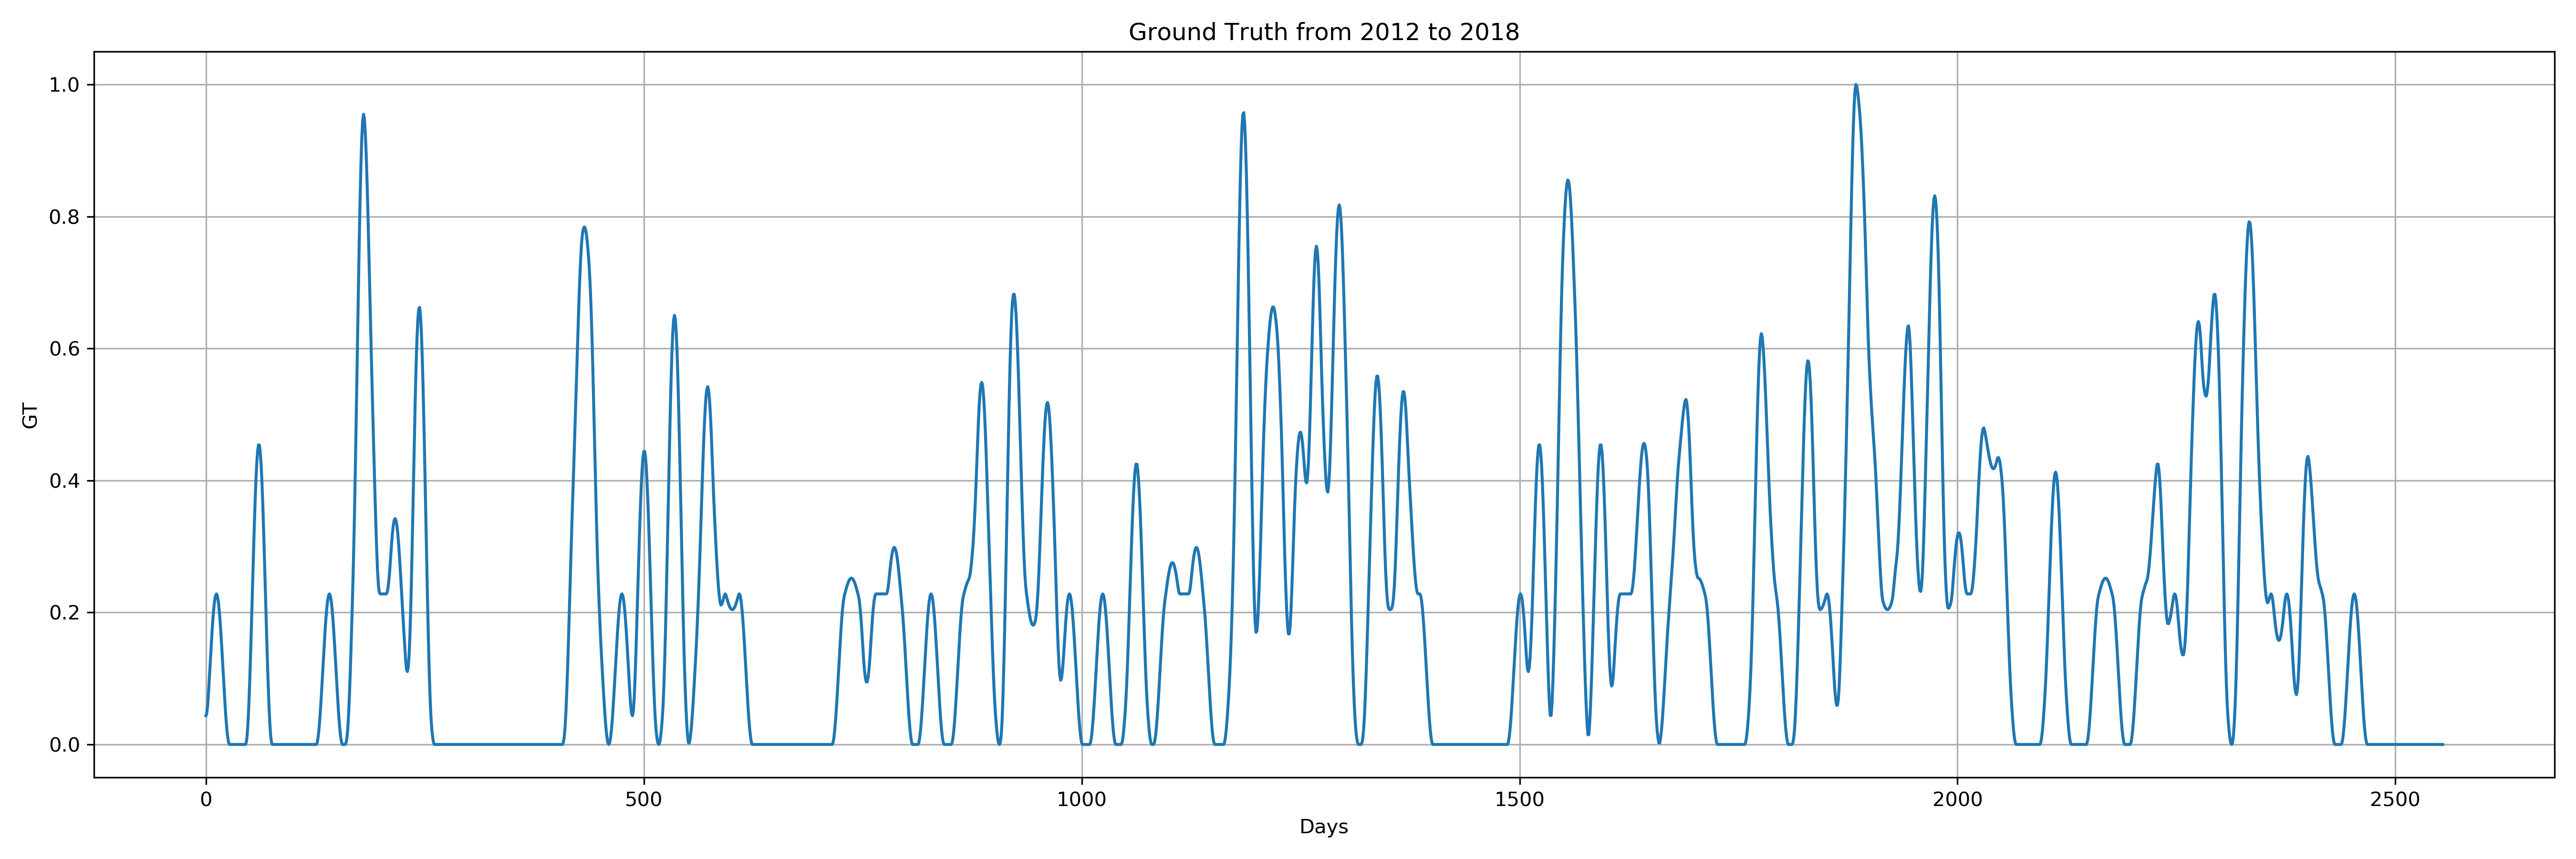
\includegraphics[width=13.2cm]{img/GT.png}
	\caption{The Figure shows an example of Ground truth generated for Florence airport from 2012 to 2018. The risk index provided by the proposed model must be very much related to the ground truth, generated by the historical events of birdstrike.}
	\label{GT_fig}
\end{figure}

\section{Model}\label{model_section}
The proposed model has been implemented using Machine Learning techniques, in particular Neural networks (Deep Learning, \ref{deep}).
Since the goal is to provide a risk value of the $K+1$ day, observing $K$ previous days, the model must work with time series. The model is based on a daily aggregation of factors, i.e. the features selected in \ref{feat_setup}, for generating the new risk-index. 
Features are embedded using a simple and learned non-linear transformation, and these embeddings are then fed into a recurrent neural network that then provides the risk value for the following day. The model uses a type of Recurrent neural network known as LSTM, \ref{LSTM_subs}.
Spearman correlation was used as accuracy to evaluate the model's performance. We did not choose it as a loss function because it is not differentiable and a loss function must be differentiable.
In order to increase the Spearman correlation between the predicted values and the ground truth, the use of multi task learning \cite{1997multitask} was chosen. To apply this approach it was necessary to design the model with the architecture of a Siamese neural network.
In the following subsections the embedding layers and the model architecture will be described.

\subsection{Embeddings}\label{embeddings_section}
A standard technique for Neural networks is to embed data into a higher- (or lower) dimensional space in order to use a learned representation of input data. 
This technique has been useful for our problem. Raw histograms are poor features for direct use in Neural networks and by using learned feature embeddings it was possible to mitigate the problem.

The embeddings size chosen for the features represented by histograms are:

\begin{itemize}
    \item Sighted Species: has been mapped from 288 dimensions down to 256 embedding dimensions.
    \item Meteorological conditions: has been mapped from 7 dimensions (all the possible weather conditions) up to 32 embedding dimensions.
    \item Temperature: has been mapped from 35 dimensions down to 32 embedding dimensions.
    \item Wind intensity: from 50 dimensions down to 16 embedding dimensions.
    \item Wind direction: from 150 dimensions down to 16 embedding dimensions.
    \item Distance to the track: from 384 dimensions down to 256 embedding dimensions.
    \item Detection environment: from 88 dimensions down to 32 embedding dimensions.
\end{itemize}
Then the resulting embeddings were concatenated with the occurrence vectors to form the final feature representation that is used as input to the LSTM layers.

\subsection{Architecture}
As mentioned previously, the core of the model is the LSTM layers and the Siamese architecture was chosen with the aim of increasing the correlation.
The model, shown in Figure \ref{architecture} is composed of two identical branches which share the same weights and architecture.
After extracting the features from the raw data in the database as discussed in section \ref{feat_setup} , the raw histograms have been embedded into embedding layers.
Then the resulting embeddings were concatenated with the occurrence vectors to form the final feature representation.
The final feature has been reshaped. The LSTM layers work with sequences and need to know what input shape they should expect.
The new shape is composed from Batch-size (number of samples that will be propagated through the network), Window (number of the days observed) and final feature.

The reshaped feature is the input for the LSTM layers. Specifically, each branch has 2 LSTM layers that sequentially process two different K-day windows. Finally, a final linear layer for each branch, with the same LSTM output size as input size, provides the risk values for the following day of the window processed.
After the embeddings layers and LSTM layers the ReLU \cite{relu} activation function was applied. And finally after the final layer the Sigmoid \cite{sigmoid} activation function was used.

The model uses a mini-batch size of 64 examples. It has been regularized by applying L2 Regularization \cite{ng2004feature} (with $\lambda = 1\times10^{-3}$), using dropout \cite{srivastava2014dropout} on the LSTM layers of 0.2 and using Adam as the Optimizer \cite{adam}.

\begin{figure}
	\centering
	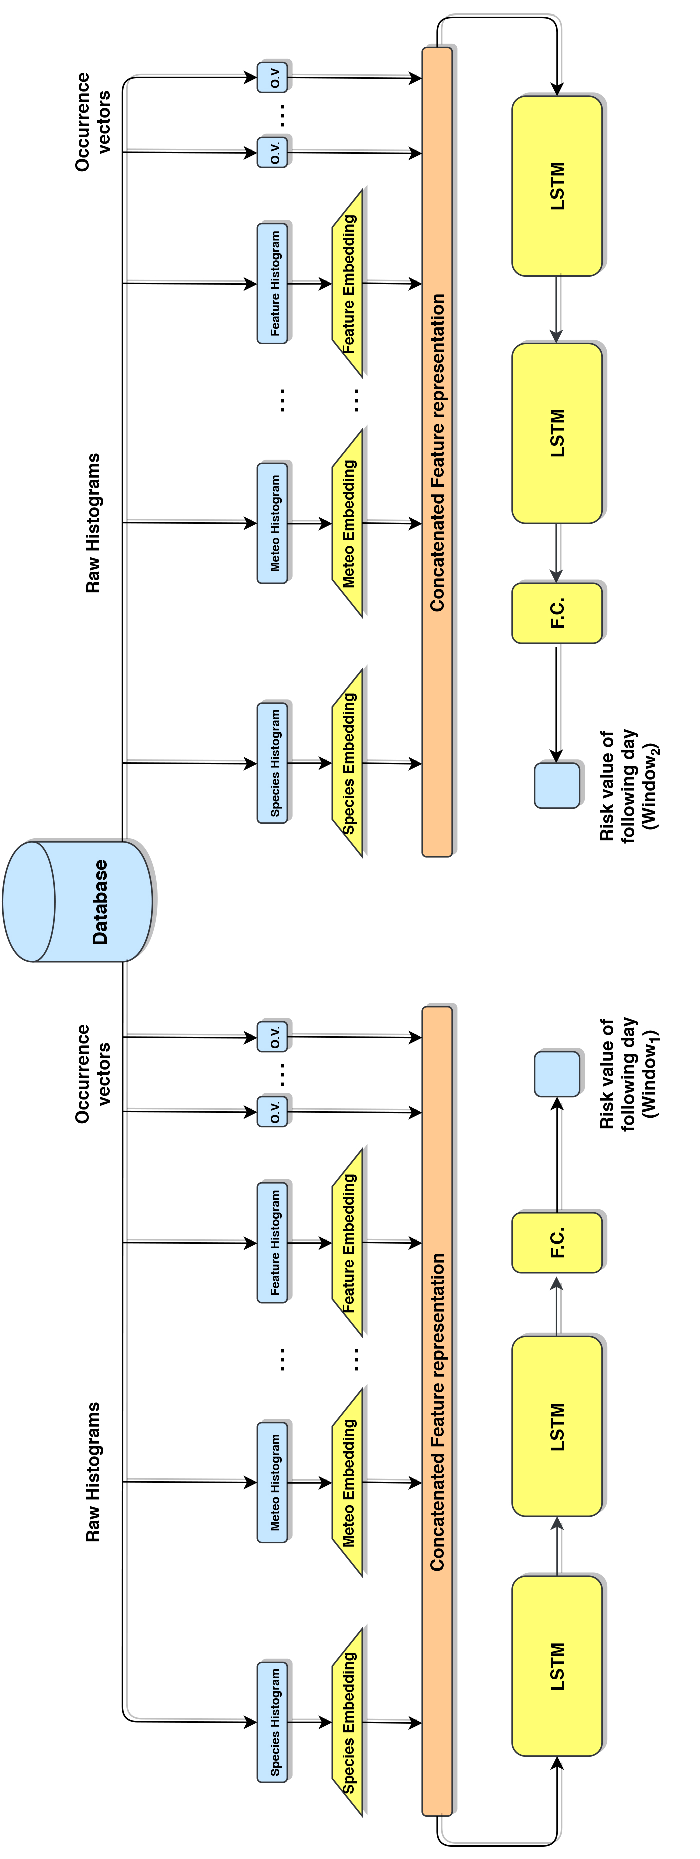
\includegraphics[width=7.3cm]{img/network2.pdf}
	\caption{The Model Architecture. Data extracted from the database are grouped by histograms and occurrence vectors. These histograms and vectors are then processed by learned embeddings (section \ref{embeddings_section}) before finally being sequentially processed by an LSTM which looks at K days of embedded factors before providing a risk-value for the following day.}
	\label{architecture}
\end{figure}

\subsection{Loss function}\label{Loss_function}
As discussed in \ref{model_section}, to improve the model's performance and generate a new risk-index more related to birdstrike events, Multi Task Learning (MTL) was chosen.
MTL help in improving the learning of the model by using the knowledge contained in two specific tasks.
The first task is to provide a risk value of the $K+1$ day, observing $K$ previous days; this is a regression problem.
The second task is to rank two risk values of two different days, i.e. the model tries to learn, given two different observation windows, which of the following two days will have higher risk.

A Custom loss function has been defined to train the model using the 2 tasks.
It takes two arguments:

\begin{itemize}
    \item Mean Absolute Error, or L1 Loss, for the first task, equation \ref{MAE}.
    \item Margin Ranking Loss (MRL), for the second task in equation \ref{MRL}.
\end{itemize}

\begin{equation}\label{MAE}
L_{MAE}(y, \hat y)=\frac{1}{N}\sum_{i=0}^N |y - \hat y|
\end{equation}

\begin{equation}\label{MRL}
L_{MRL}(y, \hat y, z) = \max(0, -z \cdot (y - \hat y) + m)
\end{equation}
where $\hat y$ is the prediction, $y$ is the Ground truth value and $z$ is the target i.e. if $z=1$ then it assumed the first input should be ranked higher (have a larger value) than the second input, and vice-versa for $z=-1$ .

Finally, the final form of the Custom loss of the model is shown in the equation \ref{custom_loss}.

\begin{equation}\label{custom_loss}
\mathcal{L}(L_{MAE}, L_{MRL})= L_{MRL} + \sigma(L_{MAE1} + L_{MAE2})
\end{equation}
where $\sigma$ is a hyperparameter, $L_{MAE1}$ and $L_{MAE2}$ are the L1 loss computed on the two network branches.

\subsubsection{Stabilization of Spearman correlation}
The Custom loss caused an unstable correlation in model training. The accuracy was found to be too sensitive to the variation of epochs, i.e. the correlation of the model would have been too dependent on the stop time.
After an ablation study on $\sigma$, a learning scheduler \cite{2012practical} was identified as a possible solution to the problem.
For some $\sigma$ values improvements were found by lowering the learning rate, and finally using the learning rate scheduler by gradually lowering the learning rate the correlation stabilized.
Specifically, the learning rate scheduler starts from a learning rate of $1 \times 10^{-5}$ and every 200 epochs is multiplied by 0.75, and the best performances were obtained with $\sigma = 0.1$.













